\section{Résultats et analyse comparative}

\subsection{Méthodologie de comparaison}
Pour valider l'implémentation de l'algorithme Parareal et évaluer sa précision, nous avons effectué une comparaison systématique avec la méthode RK4 séquentielle. Pour chaque régime dynamique (caractérisé par différentes valeurs de $\tau$), nous avons analysé :
\begin{itemize}
    \item L'évolution temporelle des trois variables (X, Y, Z)
    \item L'erreur absolue entre les solutions Parareal et RK4 pour chacune des variables.
    \item La convergence vers l'état stationnaire ou l'attracteur chaotique
    \item Les portraits de phase dans les plans X-Z, Y-Z et X-Y
\end{itemize}

\subsection{Analyse par régime dynamique}

\subsubsection{Régime non-marcheur ($\tau$ = 0.5)}
Pour le régime de faible mémoire, où le système converge vers un point fixe :

\begin{figure}[H]
    \centering
    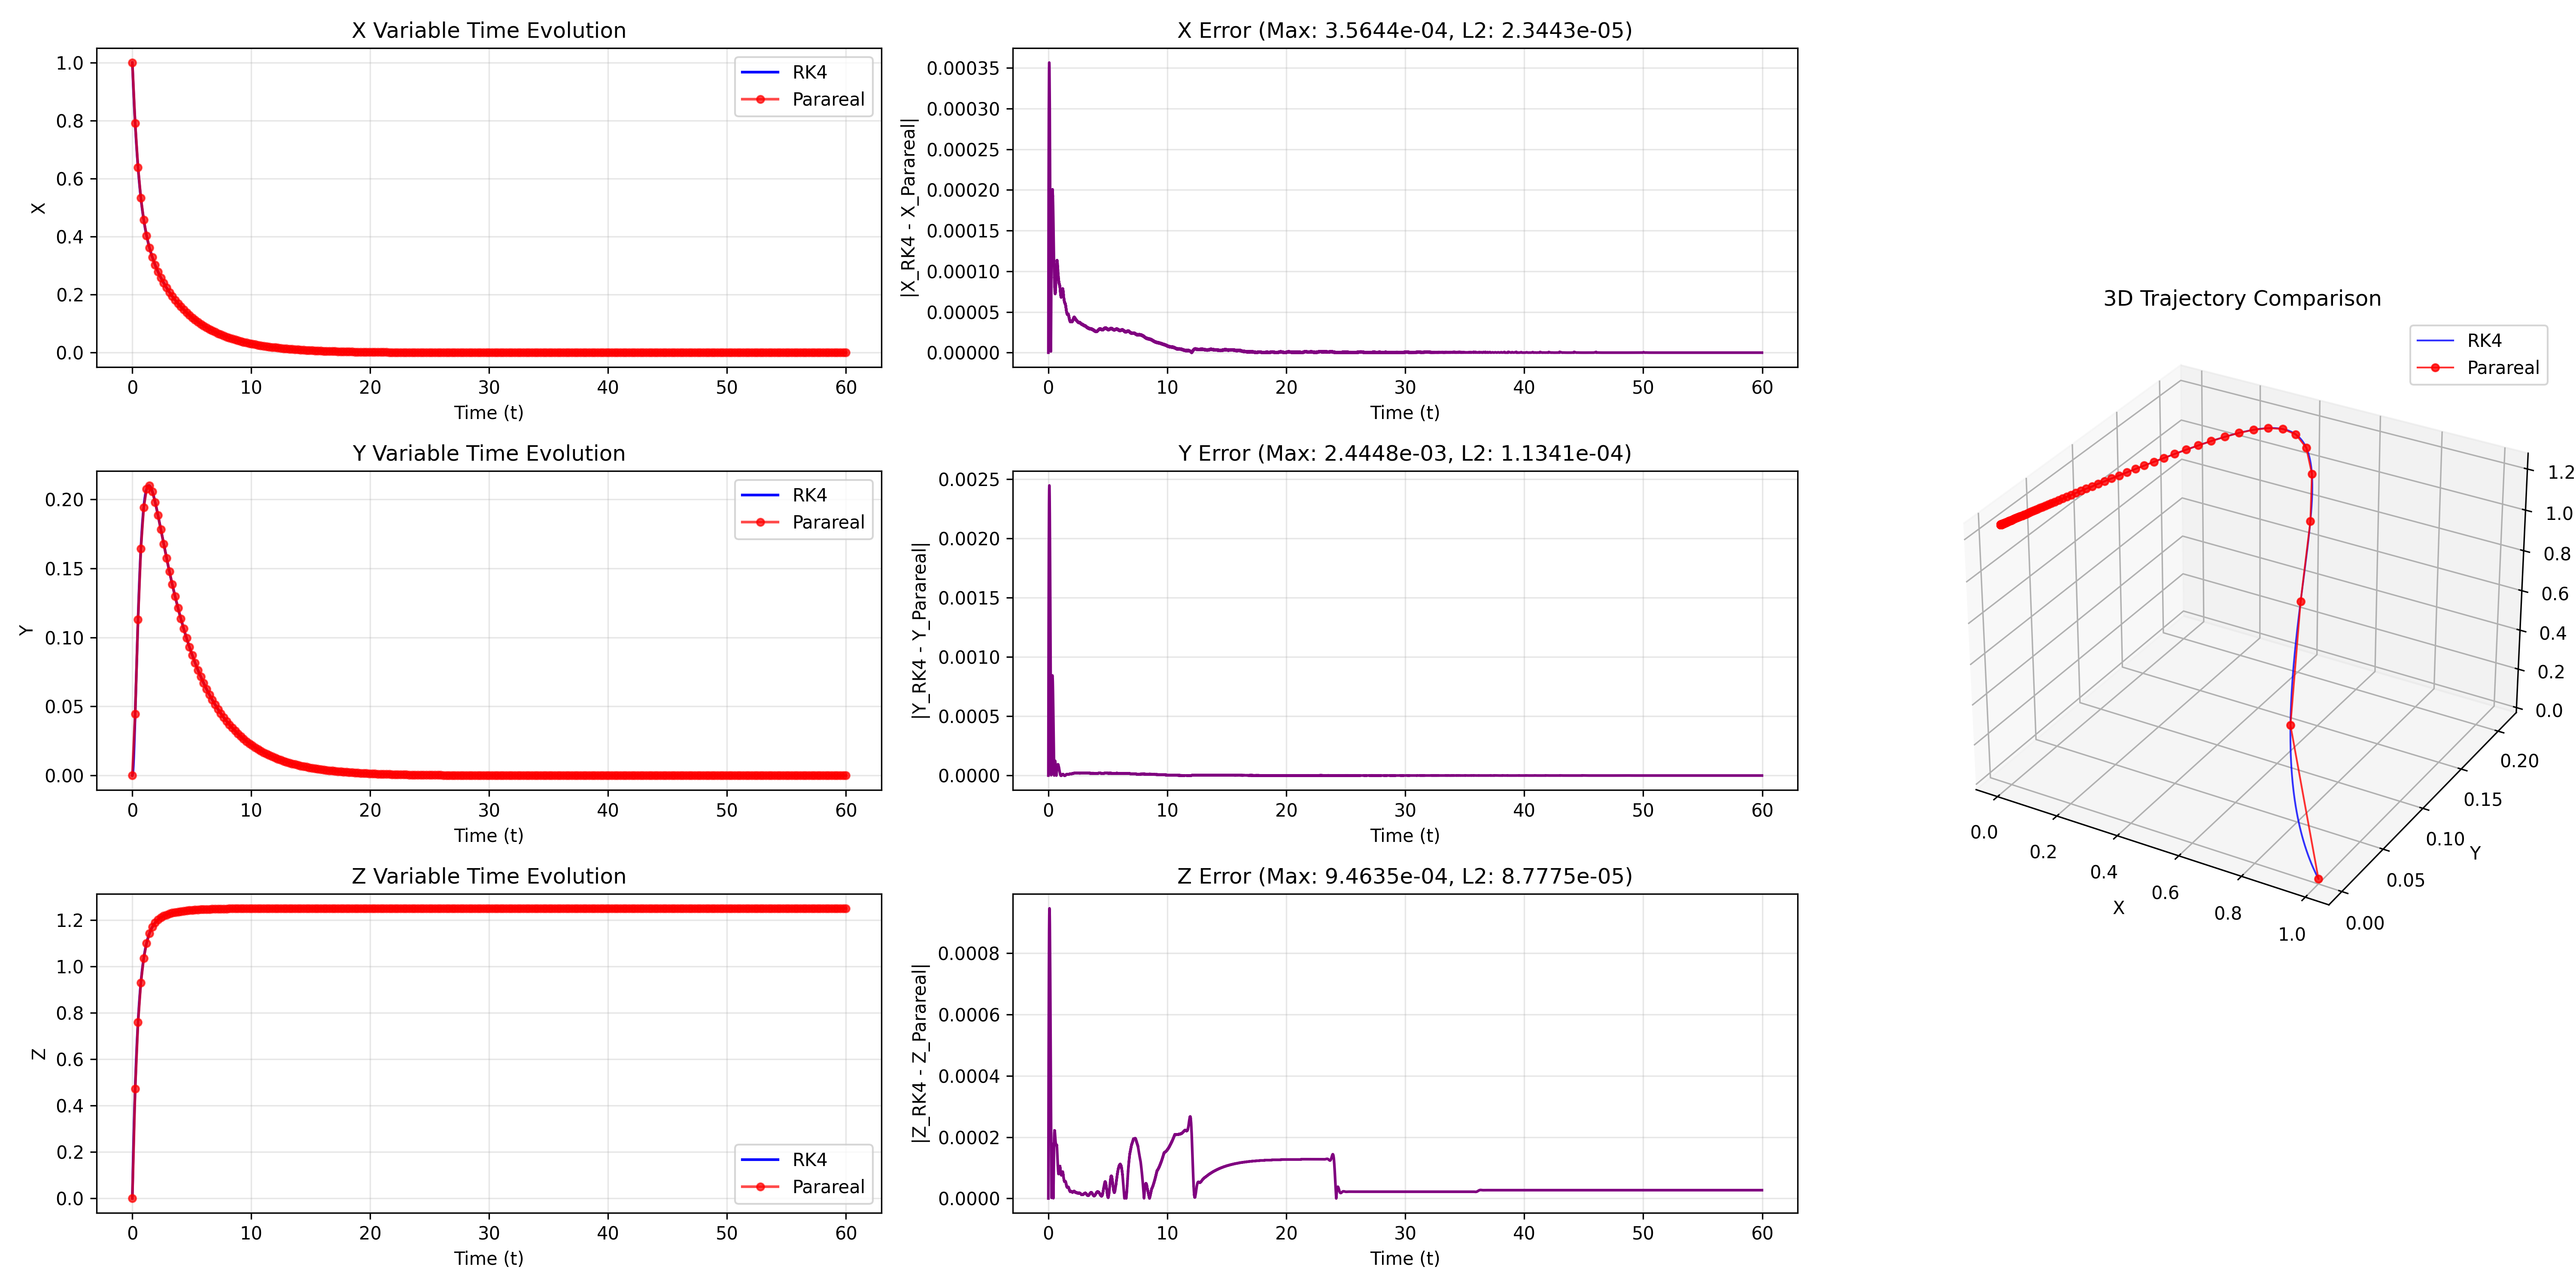
\includegraphics[width=\textwidth]{figures/comparisons/comparison_tau0.5_comparison}
    \caption{Comparaison des évolutions temporelles et erreurs temporelles pour $\tau$ = 0.5}
    \label{fig:comp_tau0.5_time}
\end{figure}

Les résultats montrent :
\begin{itemize}
    \item Une excellente concordance entre les deux méthodes dans la prédiction de la convergence vers l'origine
    \item Des erreurs absolues très faibles ($< 10^{-6}$) après la phase transitoire initiale
    \item Une stabilité numérique comparable pour les deux approches
\end{itemize}

\begin{figure}[H]
    \centering
    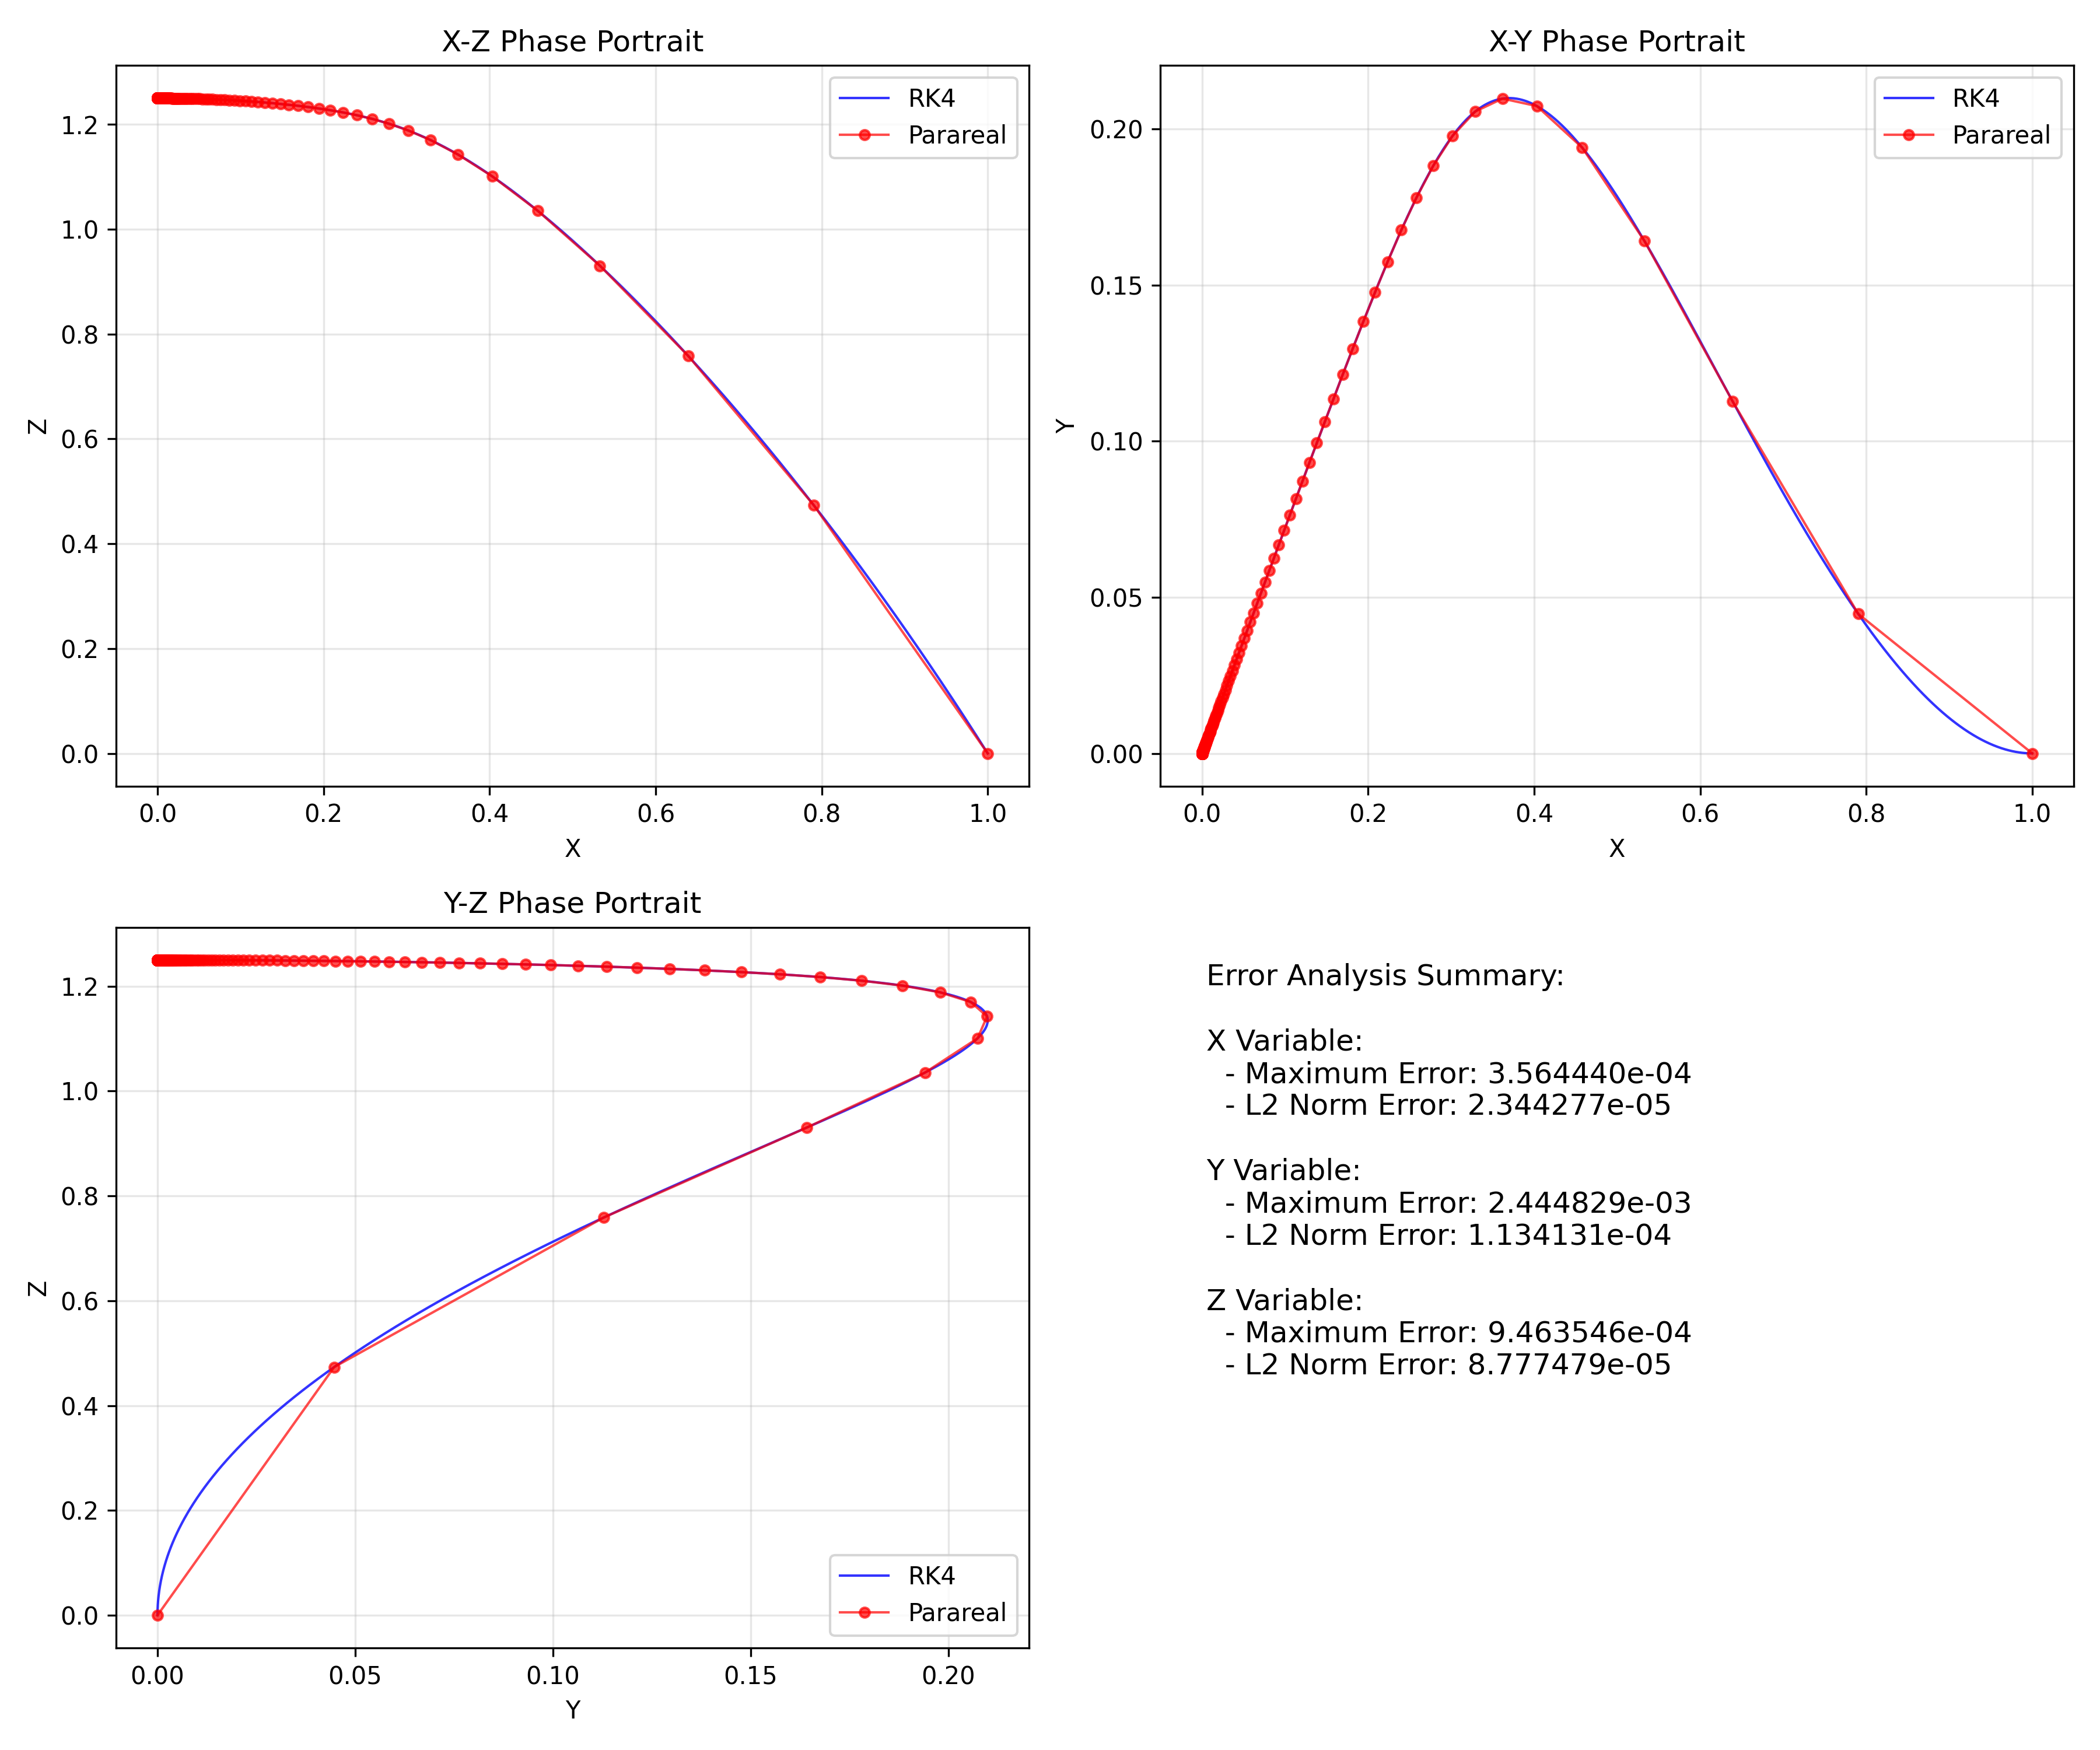
\includegraphics[width=\textwidth]{figures/comparisons/comparison_tau0.5_phase_portraits}
    \caption{Portraits de phase comparés pour $\tau$ = 0.5}
    \label{fig:comp_tau0.5_phase}
\end{figure}

Les portraits de phase confirment la précision de l'algorithme Parareal dans la capture de la dynamique de convergence.

\subsubsection{Régime de marche régulière ($\tau$ = 2.0)}
Pour le régime de marche stable :

\begin{figure}[H]
    \centering
    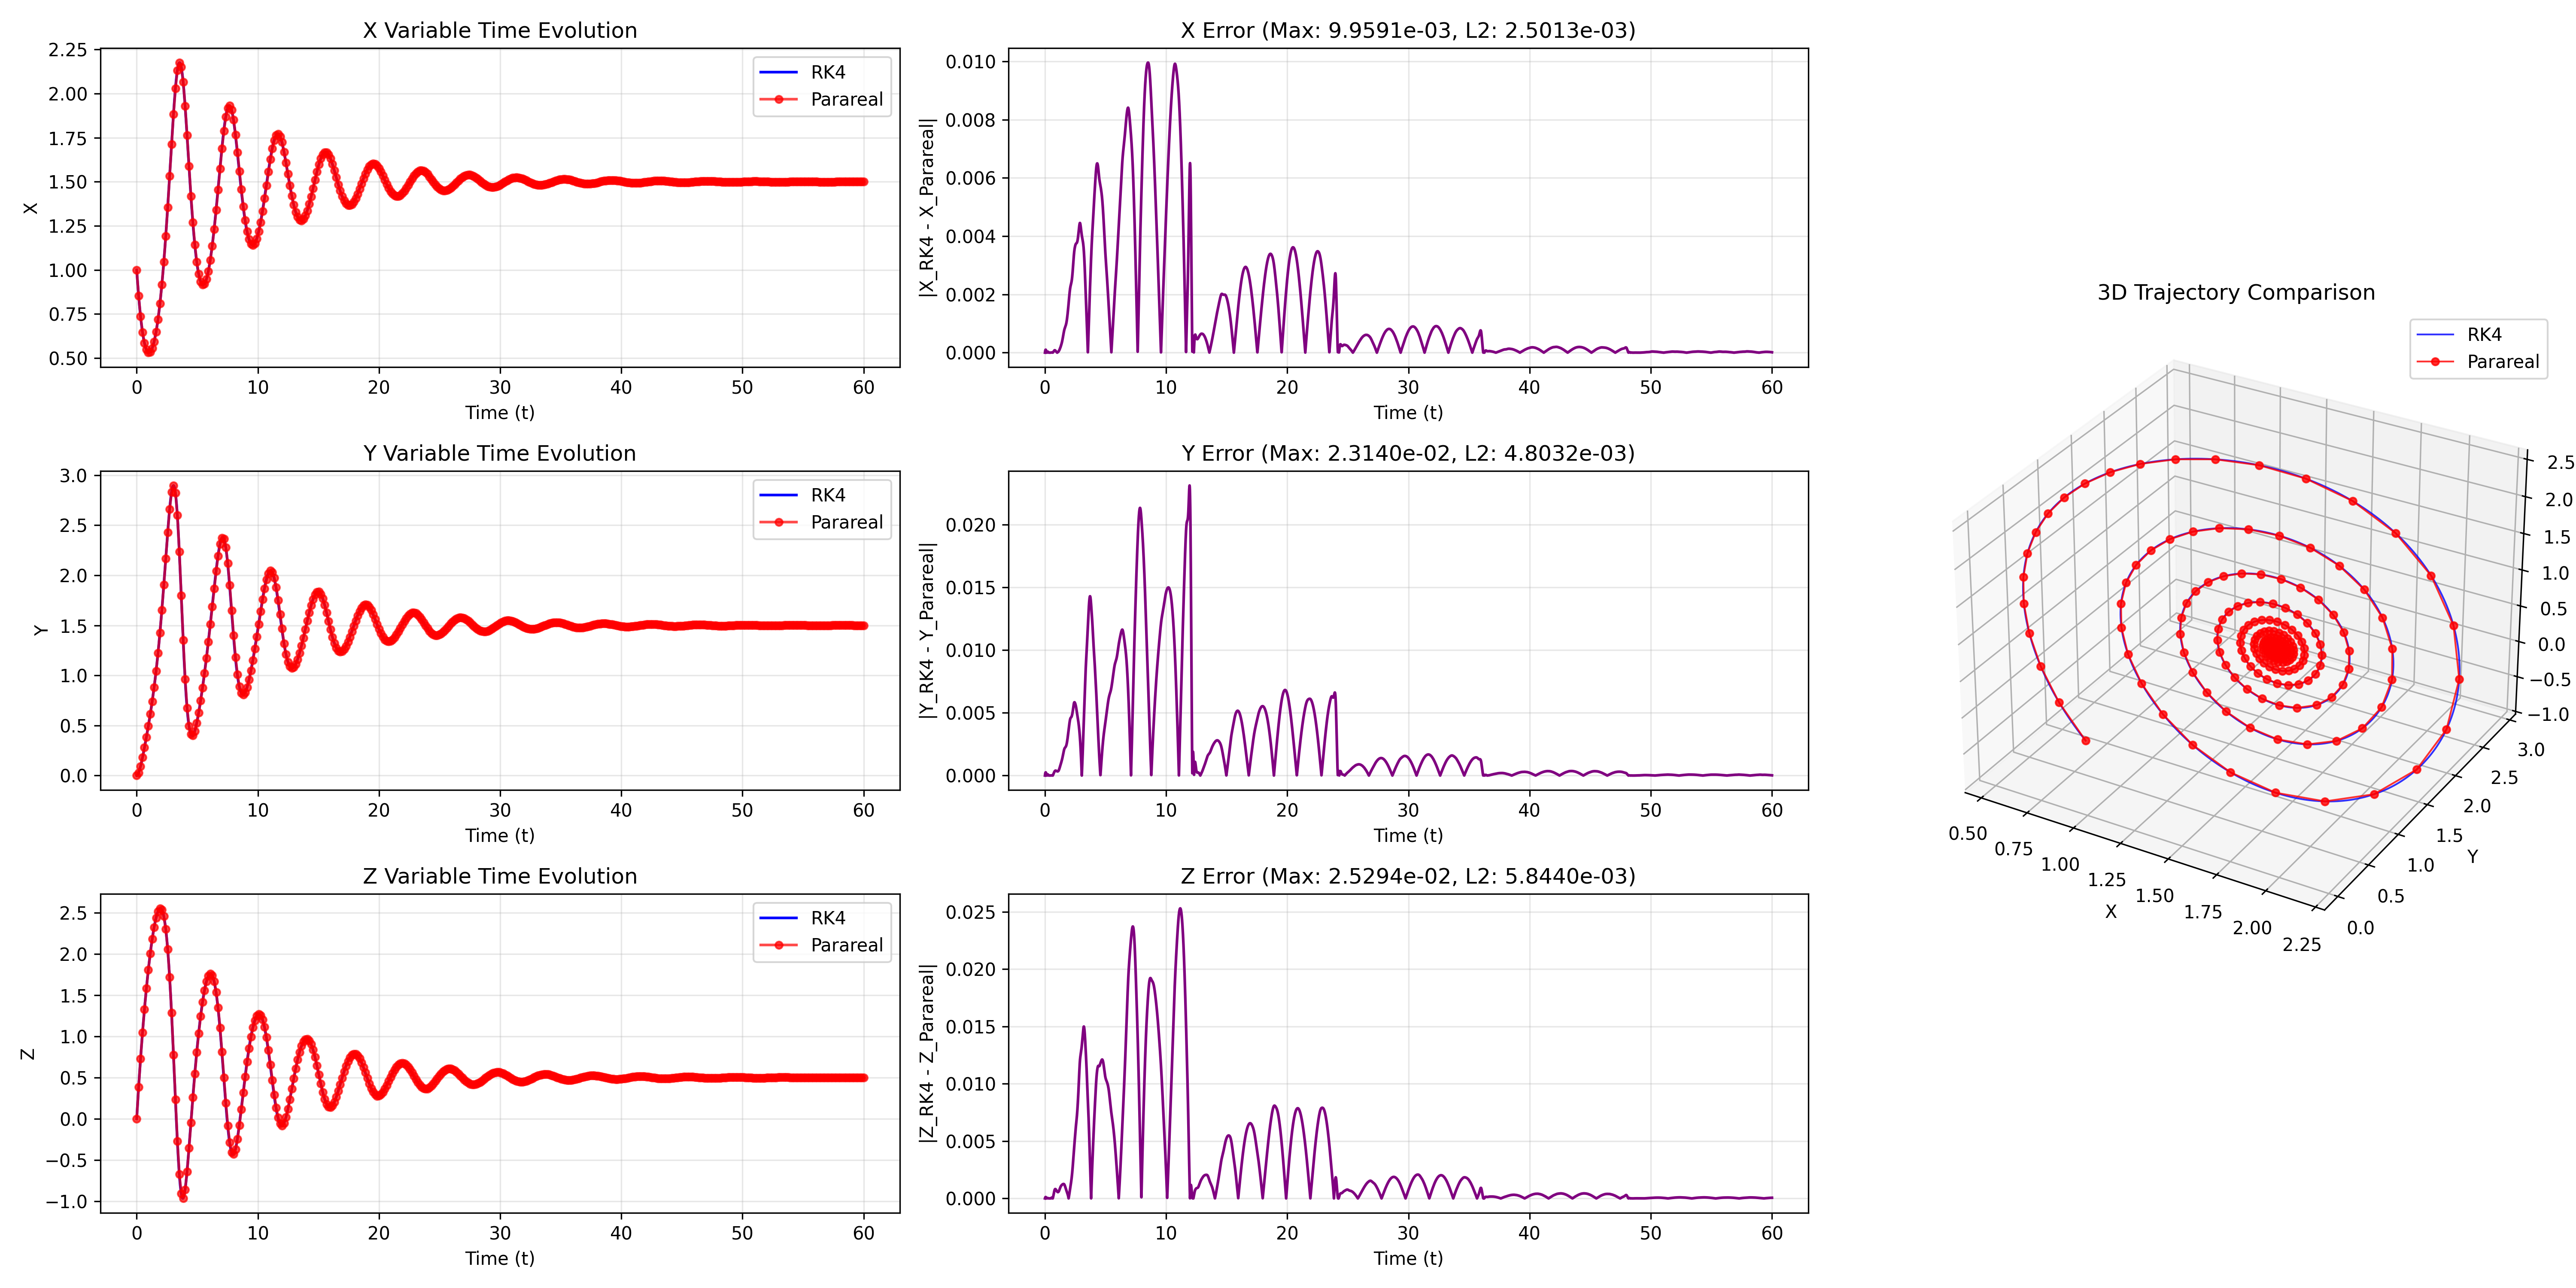
\includegraphics[width=\textwidth]{figures/comparisons/comparison_tau2.0_comparison}
    \caption{Comparaison des évolutions temporelles et erreurs absolues pour $\tau$ = 2.0}
    \label{fig:comp_tau2.0_time}
\end{figure}

L'analyse révèle :
\begin{itemize}
    \item Une reproduction fidèle des états stationnaires non-triviaux
    \item Une stabilisation rapide des erreurs à des niveaux très bas
    \item Une capacité à maintenir la précision sur de longues durées de simulation
\end{itemize}

\begin{figure}[H]
    \centering
    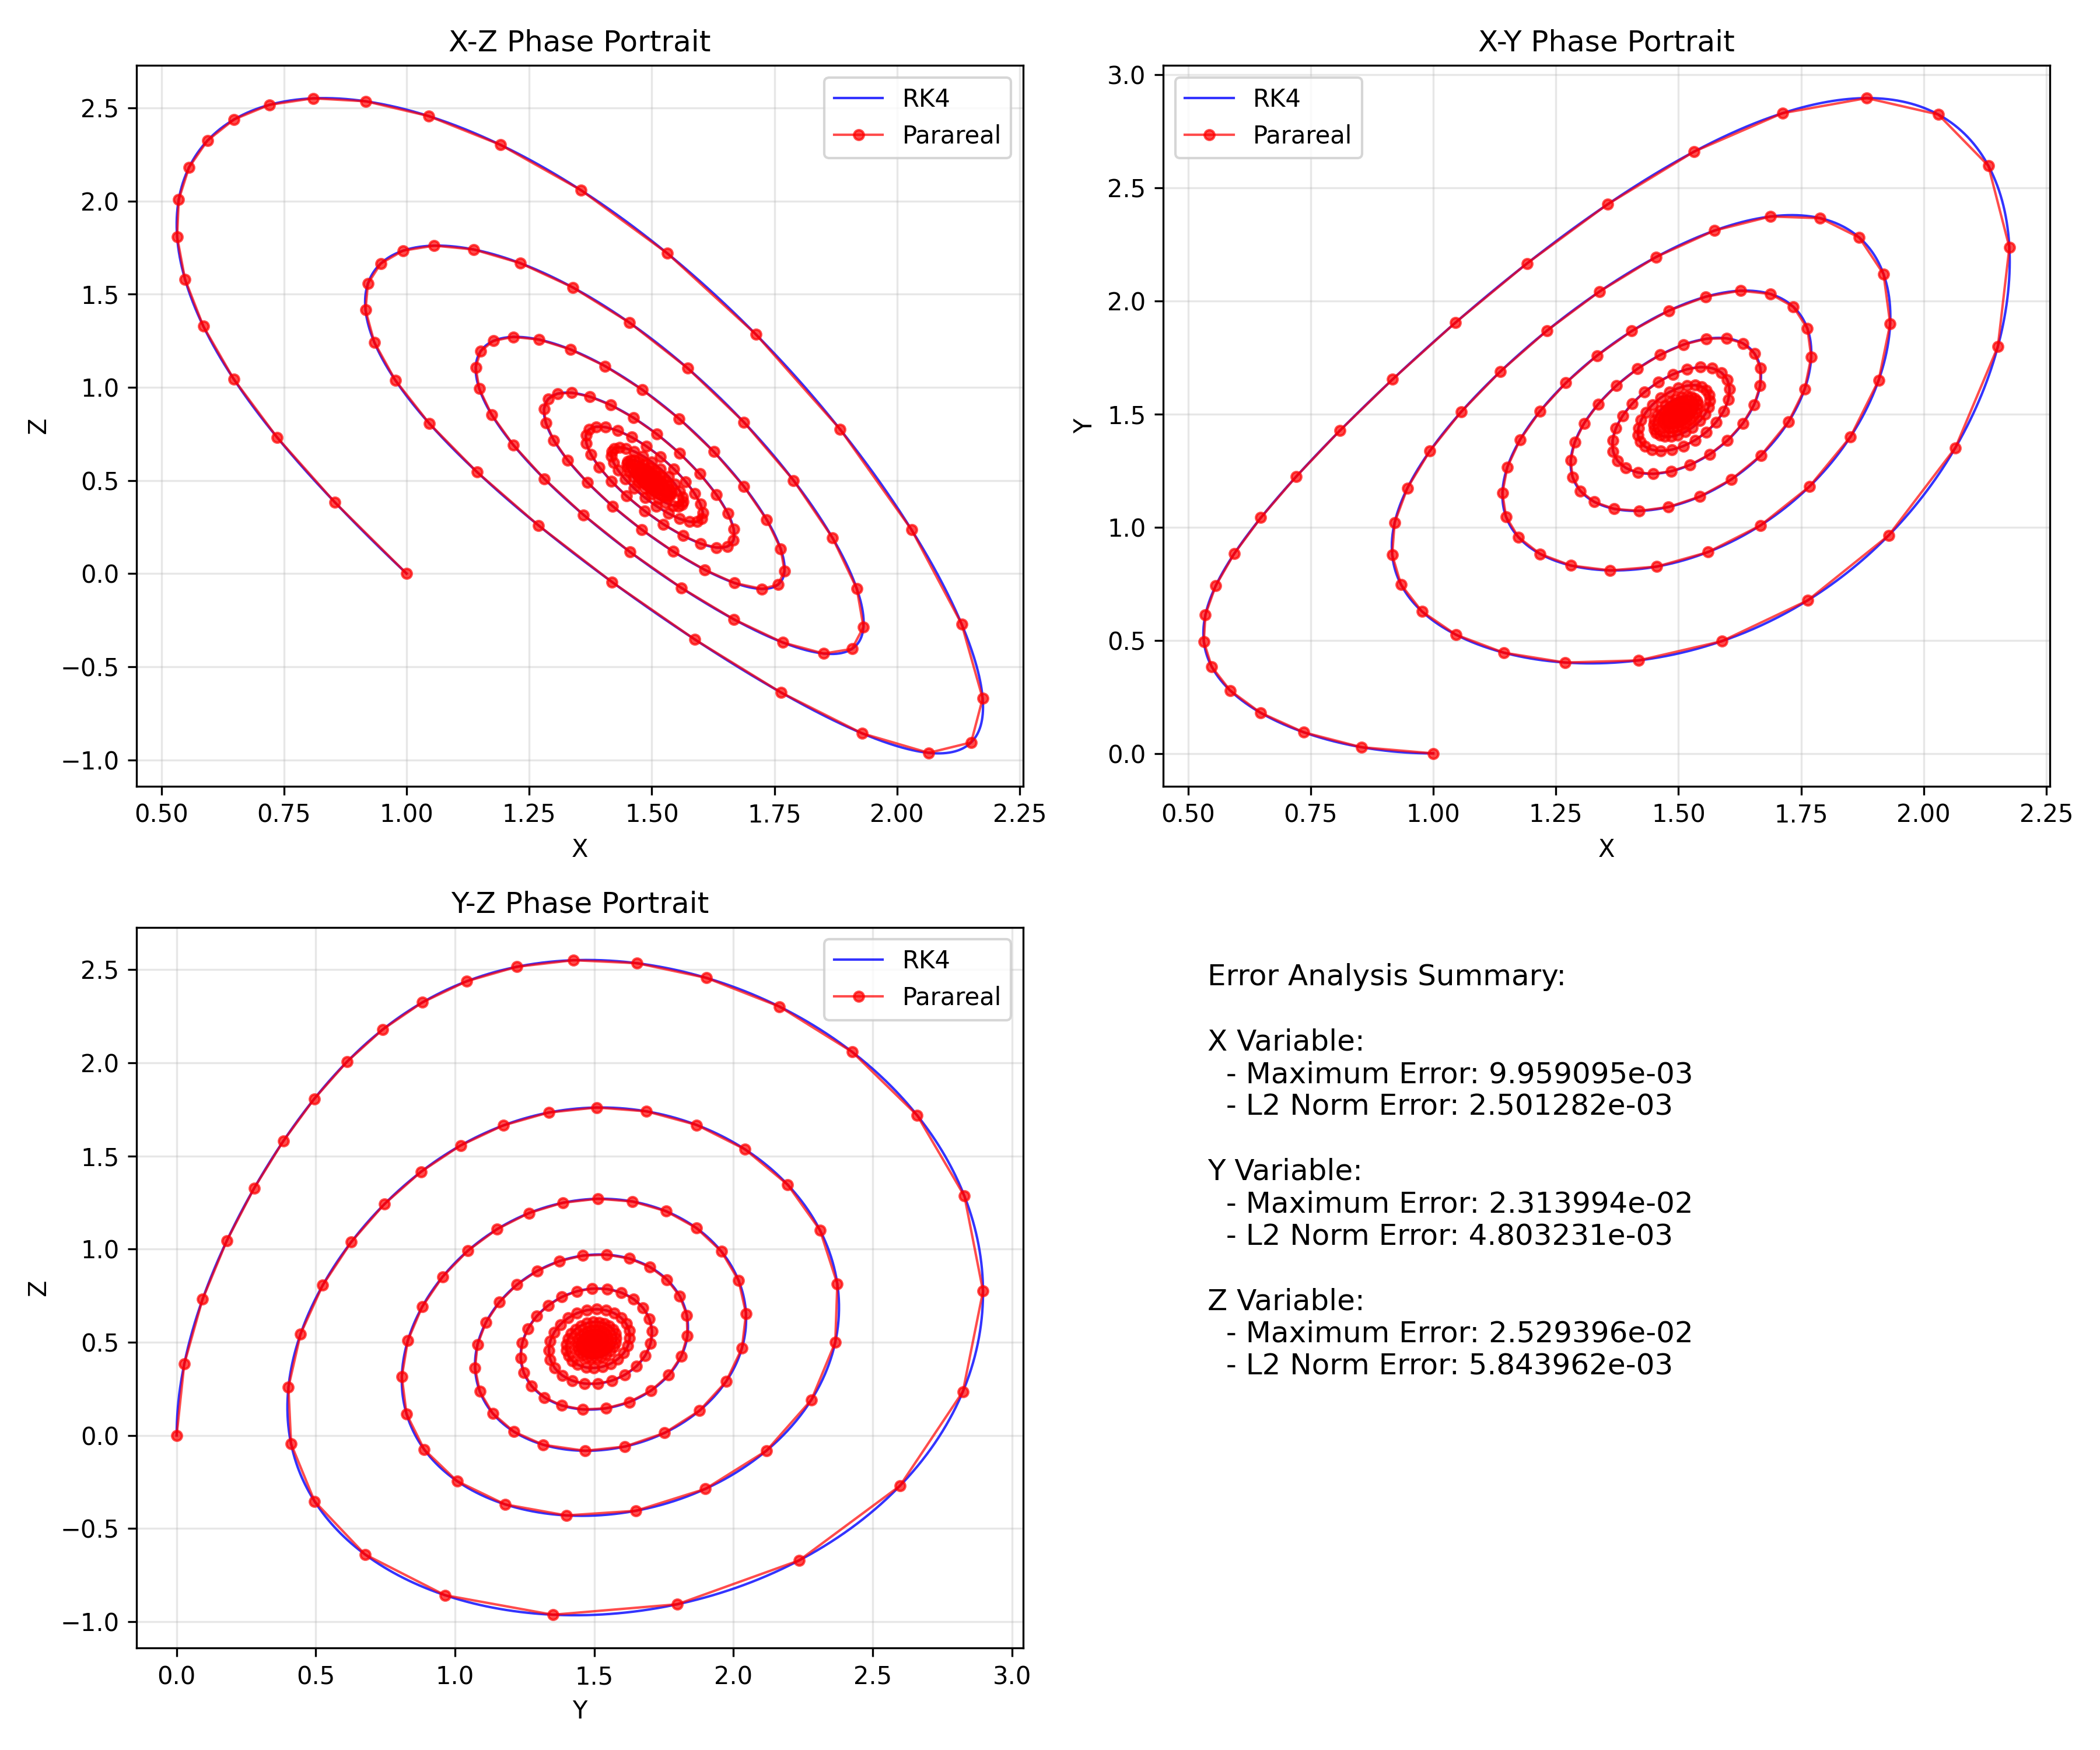
\includegraphics[width=\textwidth]{figures/comparisons/comparison_tau2.0_phase_portraits}
    \caption{Portraits de phase comparés pour $\tau$ = 2.0}
    \label{fig:comp_tau2.0_phase}
\end{figure}

Les trajectoires dans l'espace des phases sont pratiquement indiscernables entre les deux méthodes.

\subsubsection{Régime chaotique ($\tau$ = 5.0)}
Dans le régime de forte non-linéarité :

\begin{figure}[H]
    \centering
    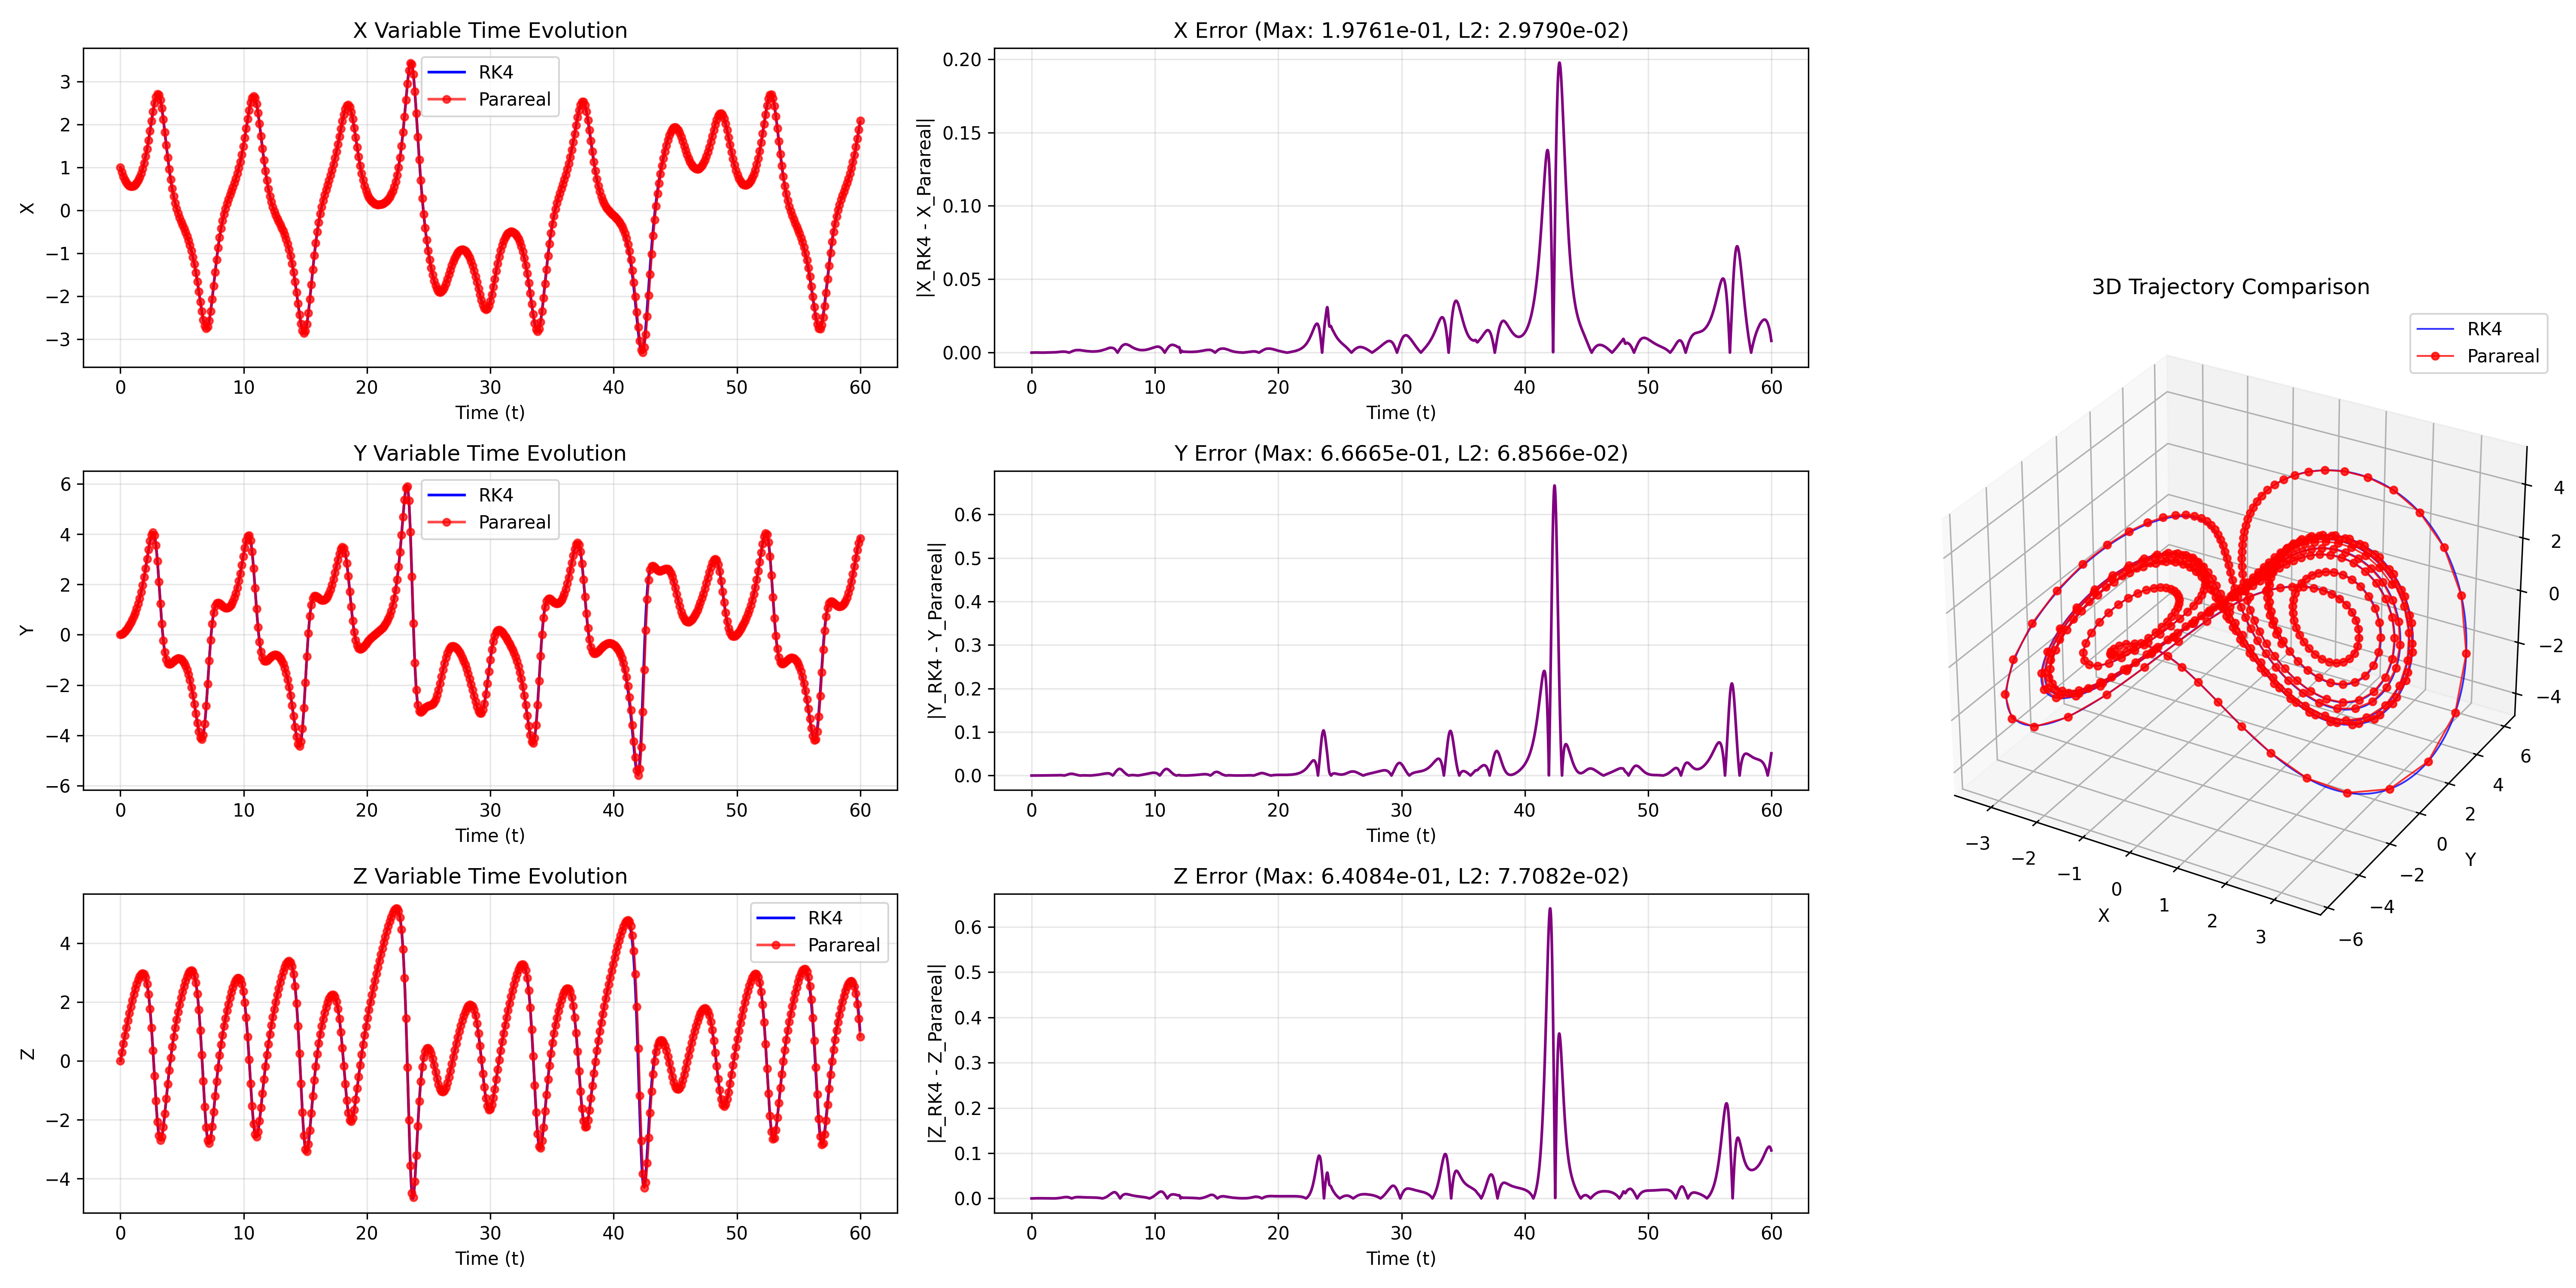
\includegraphics[width=\textwidth]{figures/comparisons/comparison_tau5.0_comparison}
    \caption{Comparaison des évolutions temporelles et erreurs absolues pour $\tau$ = 5.0}
    \label{fig:comp_tau5.0_time}
\end{figure}

Observations principales :
\begin{itemize}
    \item Les trajectoires restent cohérentes malgré la nature chaotique du système
    \item Les erreurs absolues montrent des pics correspondant aux transitions dynamiques
    \item La structure globale de l'attracteur est préservée
\end{itemize}

\begin{figure}[H]
    \centering
    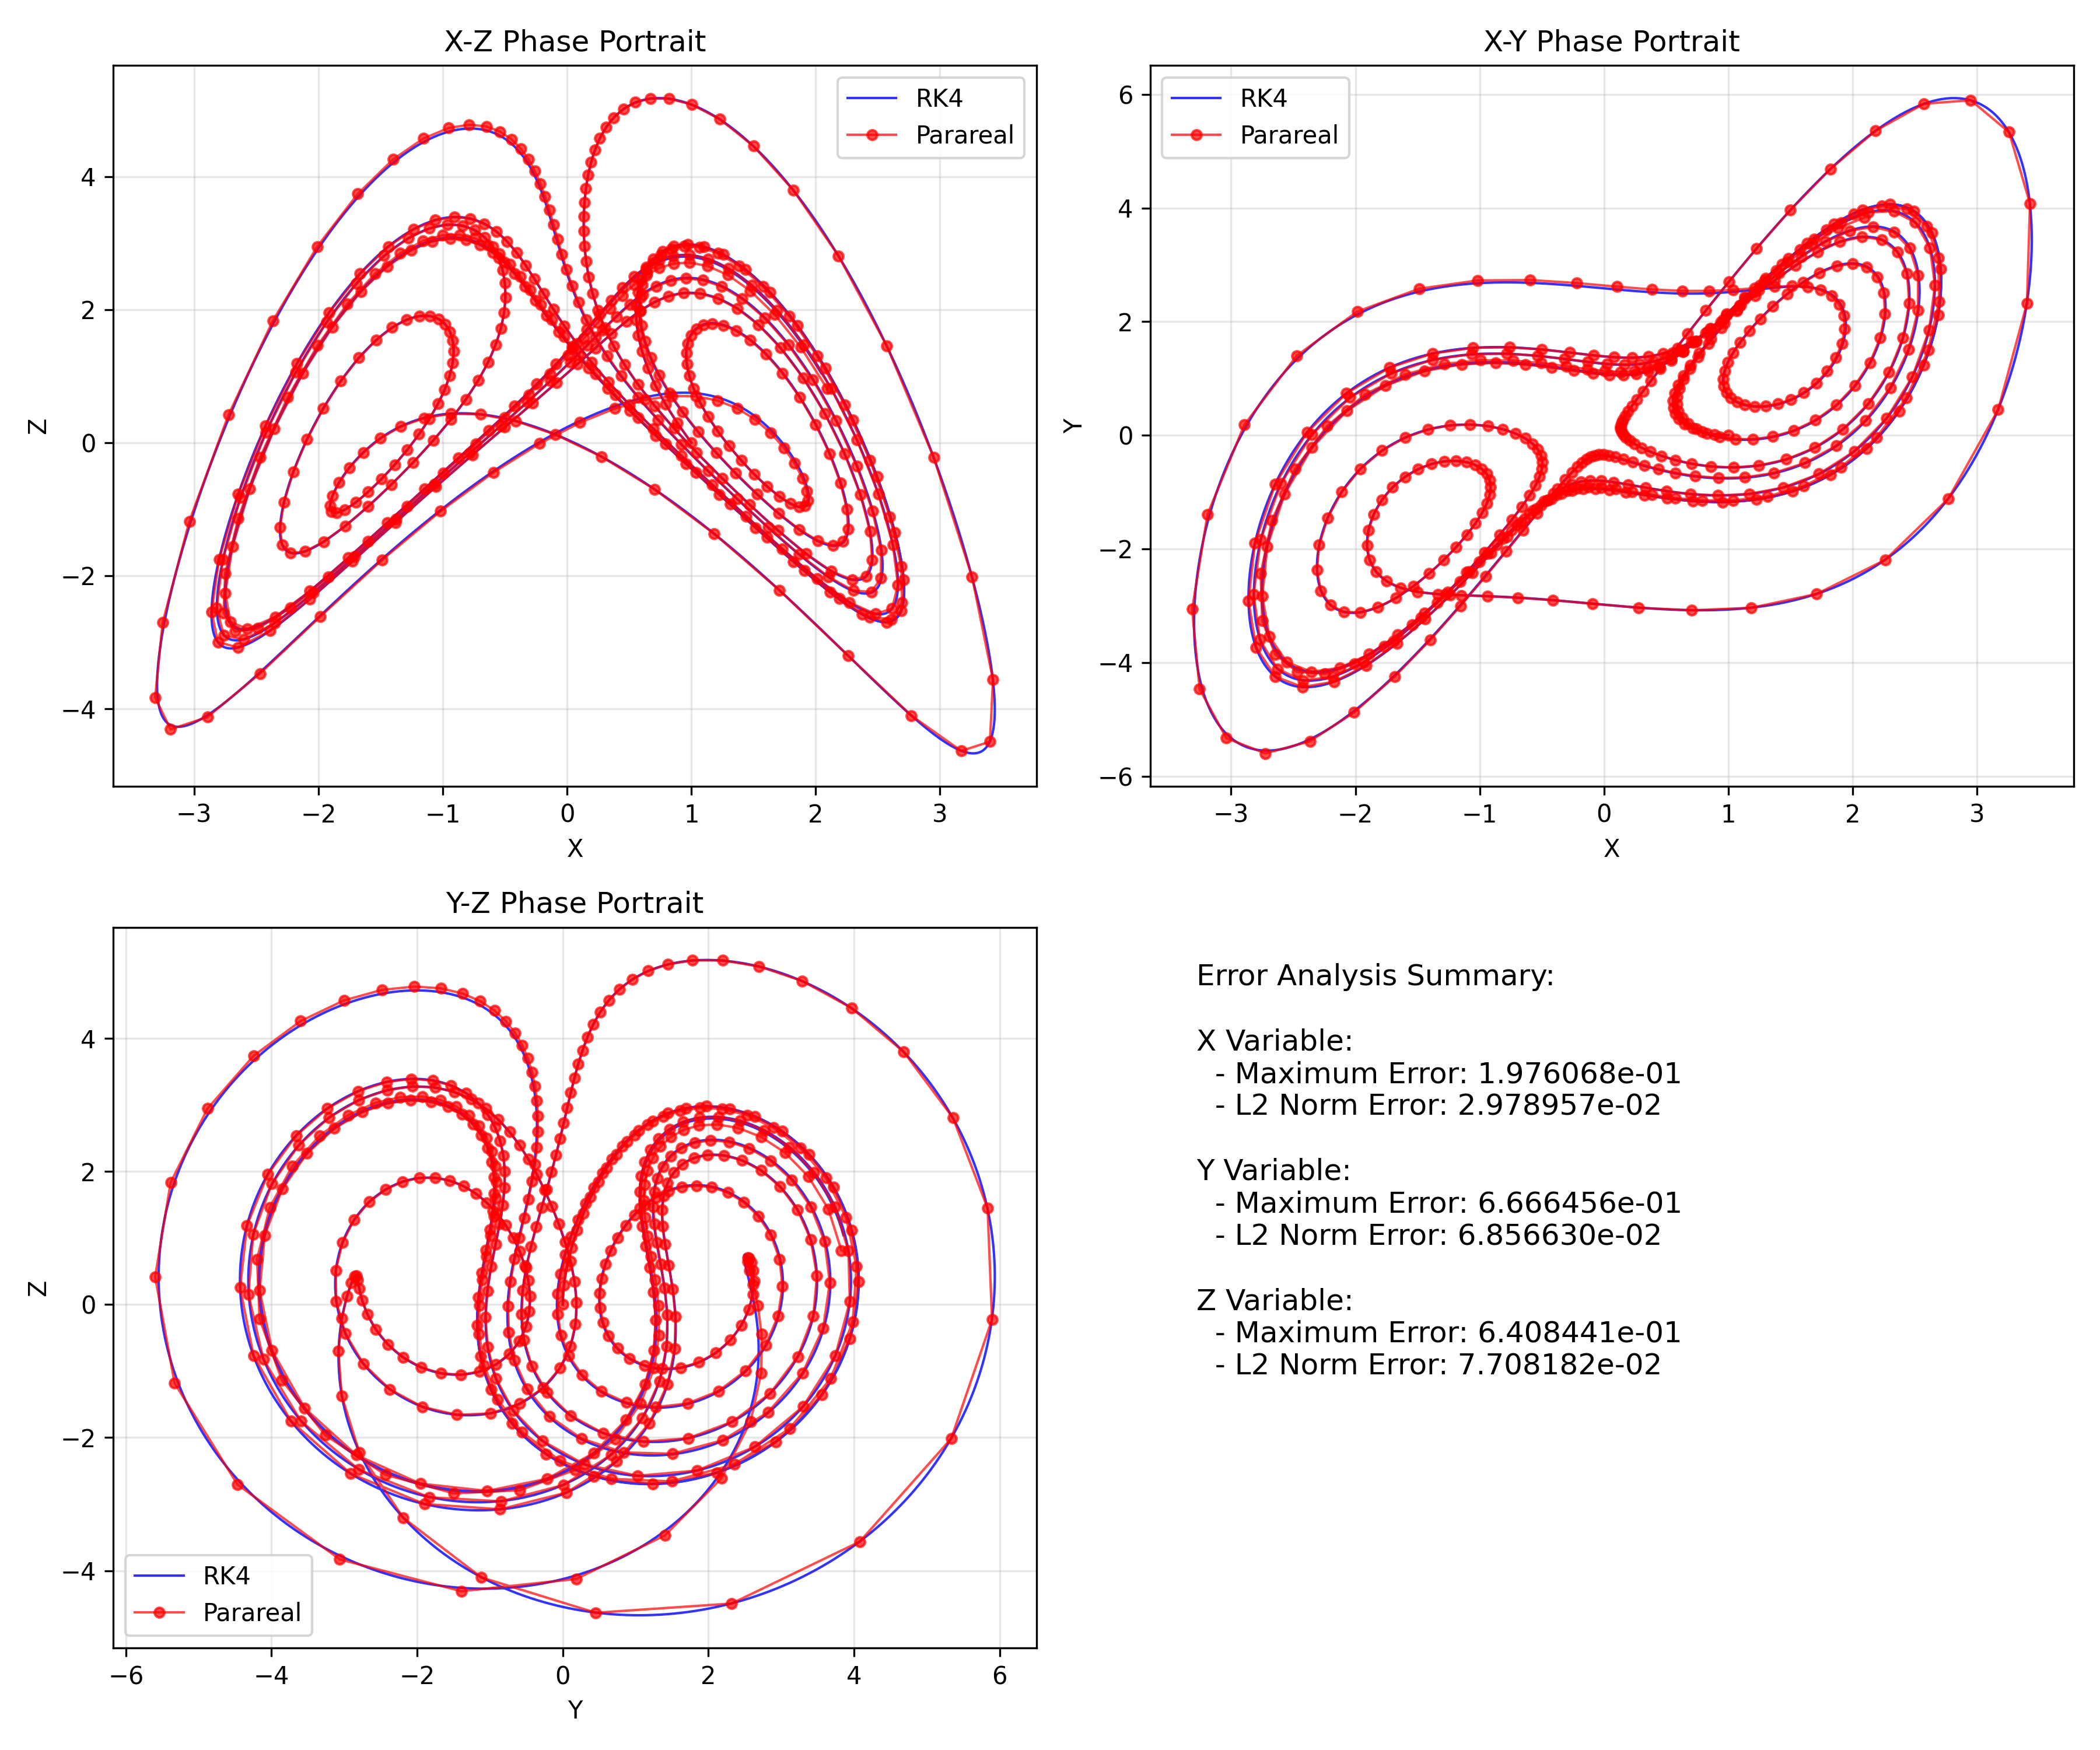
\includegraphics[width=\textwidth]{figures/comparisons/comparison_tau5.0_phase_portraits}
    \caption{Portraits de phase comparés pour $\tau$ = 5.0}
    \label{fig:comp_tau5.0_phase}
\end{figure}

Les portraits de phase démontrent la capacité de l'algorithme Parareal à reproduire la structure complexe de l'attracteur étrange.

\subsection{Synthèse des performances}

La comparaison systématique des résultats permet de conclure que :

\begin{itemize}
    % \item \textbf{Précision} :
    % \begin{itemize}
    \item Erreurs relatives maintenues sous $10^{-4}$ pour les régimes stables
    \item Reproduction fidèle des caractéristiques qualitatives dans les régimes chaotiques
    \item Conservation des invariants du système
    % \end{itemize}
    
    % \item \textbf{Stabilité} :
    % \begin{itemize}
    %     \item Aucune divergence observée, même dans les régimes fortement non-linéaires
    %     \item Robustesse face aux transitions dynamiques
    %     \item Maintien de la précision sur de longues durées de simulation
    % \end{itemize}
    
\end{itemize}

Ces résultats valident l'approche Parareal comme une alternative viable à RK4 pour la simulation du système de Lorenz, offrant un compromis optimal entre précision et performance grâce à la parallélisation temporelle.

\subsection{Analyse des performances}

\subsubsection{Performances temporelles}
\begin{itemize}
    \item \textbf{Accélération} : Gain significatif avec une réduction significative du temps de calcul
    \item \textbf{Efficacité} : Maintien d'une efficacité supérieure à 50\% même à grande échelle
    \item \textbf{Scalabilité} : Comportement quasi-linéaire jusqu'à 250000 itérations
\end{itemize}

\begin{figure}[h]
    \centering
    \begin{subfigure}[b]{0.48\textwidth}
        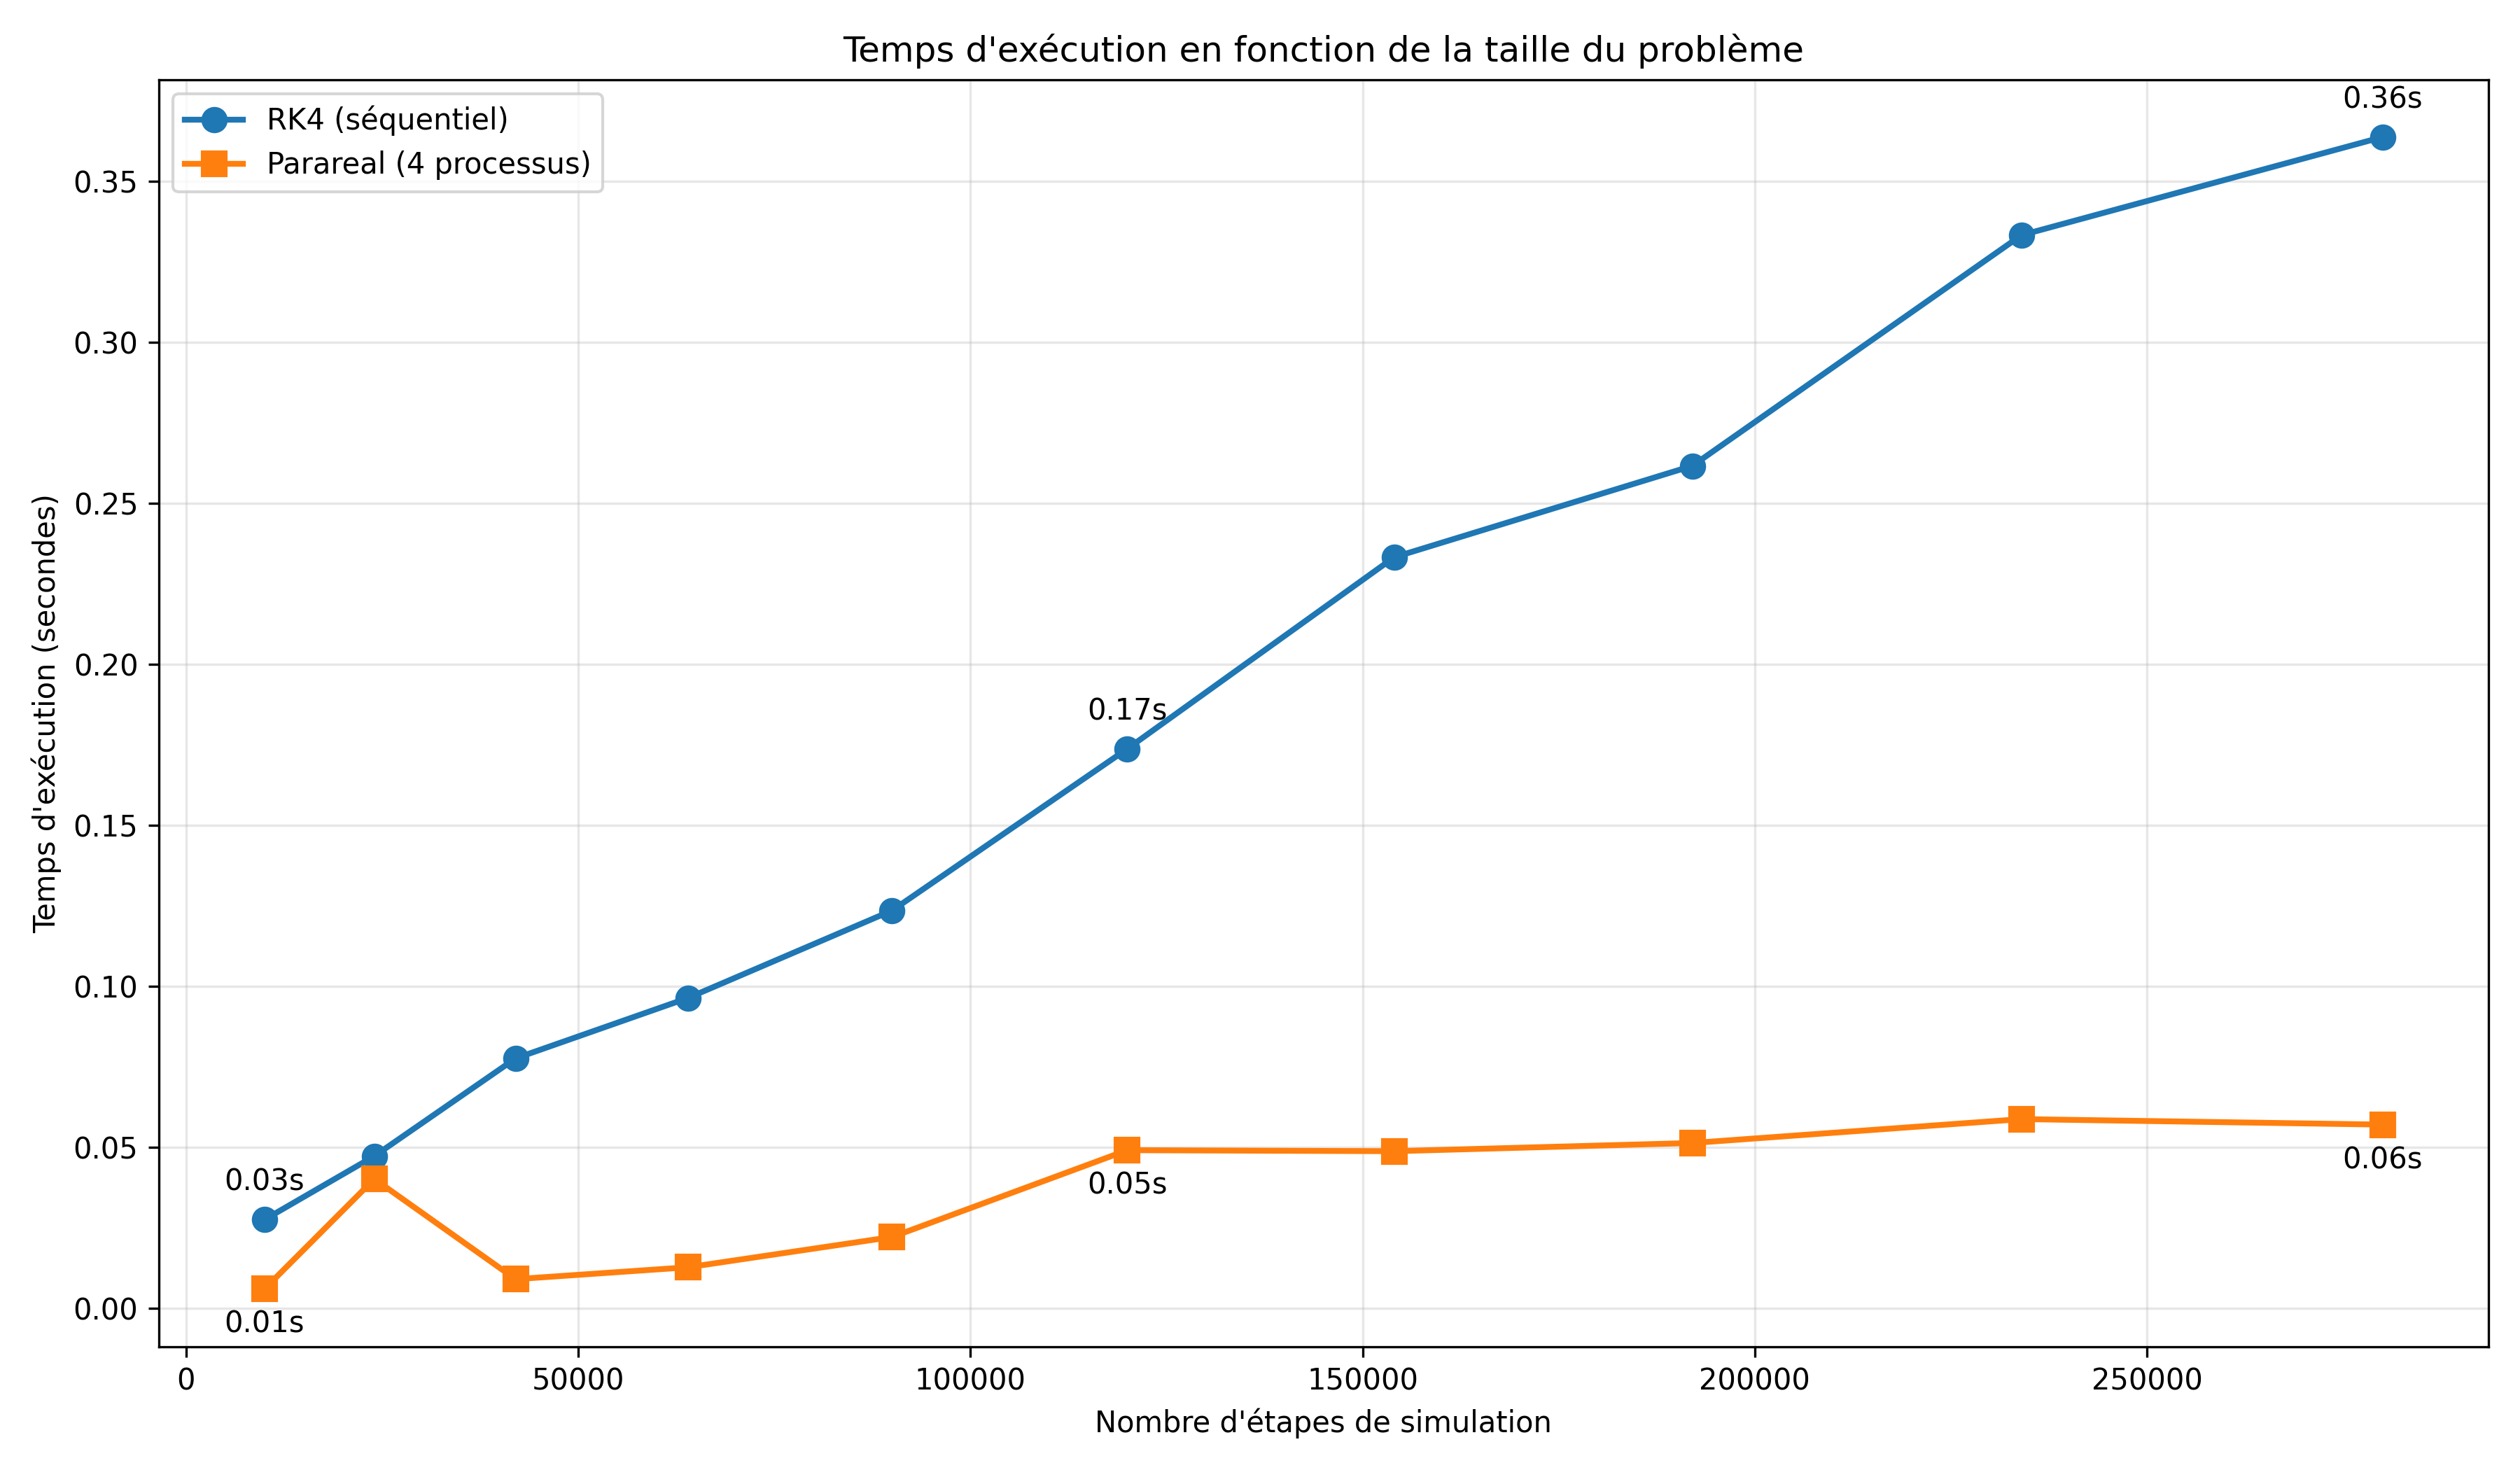
\includegraphics[width=\textwidth]{figures/benchmarks/execution_time_steps}
        \caption{Temps d'exécution par pas de temps}
        \label{fig:exec_time}
    \end{subfigure}
    \begin{subfigure}[b]{0.48\textwidth}
        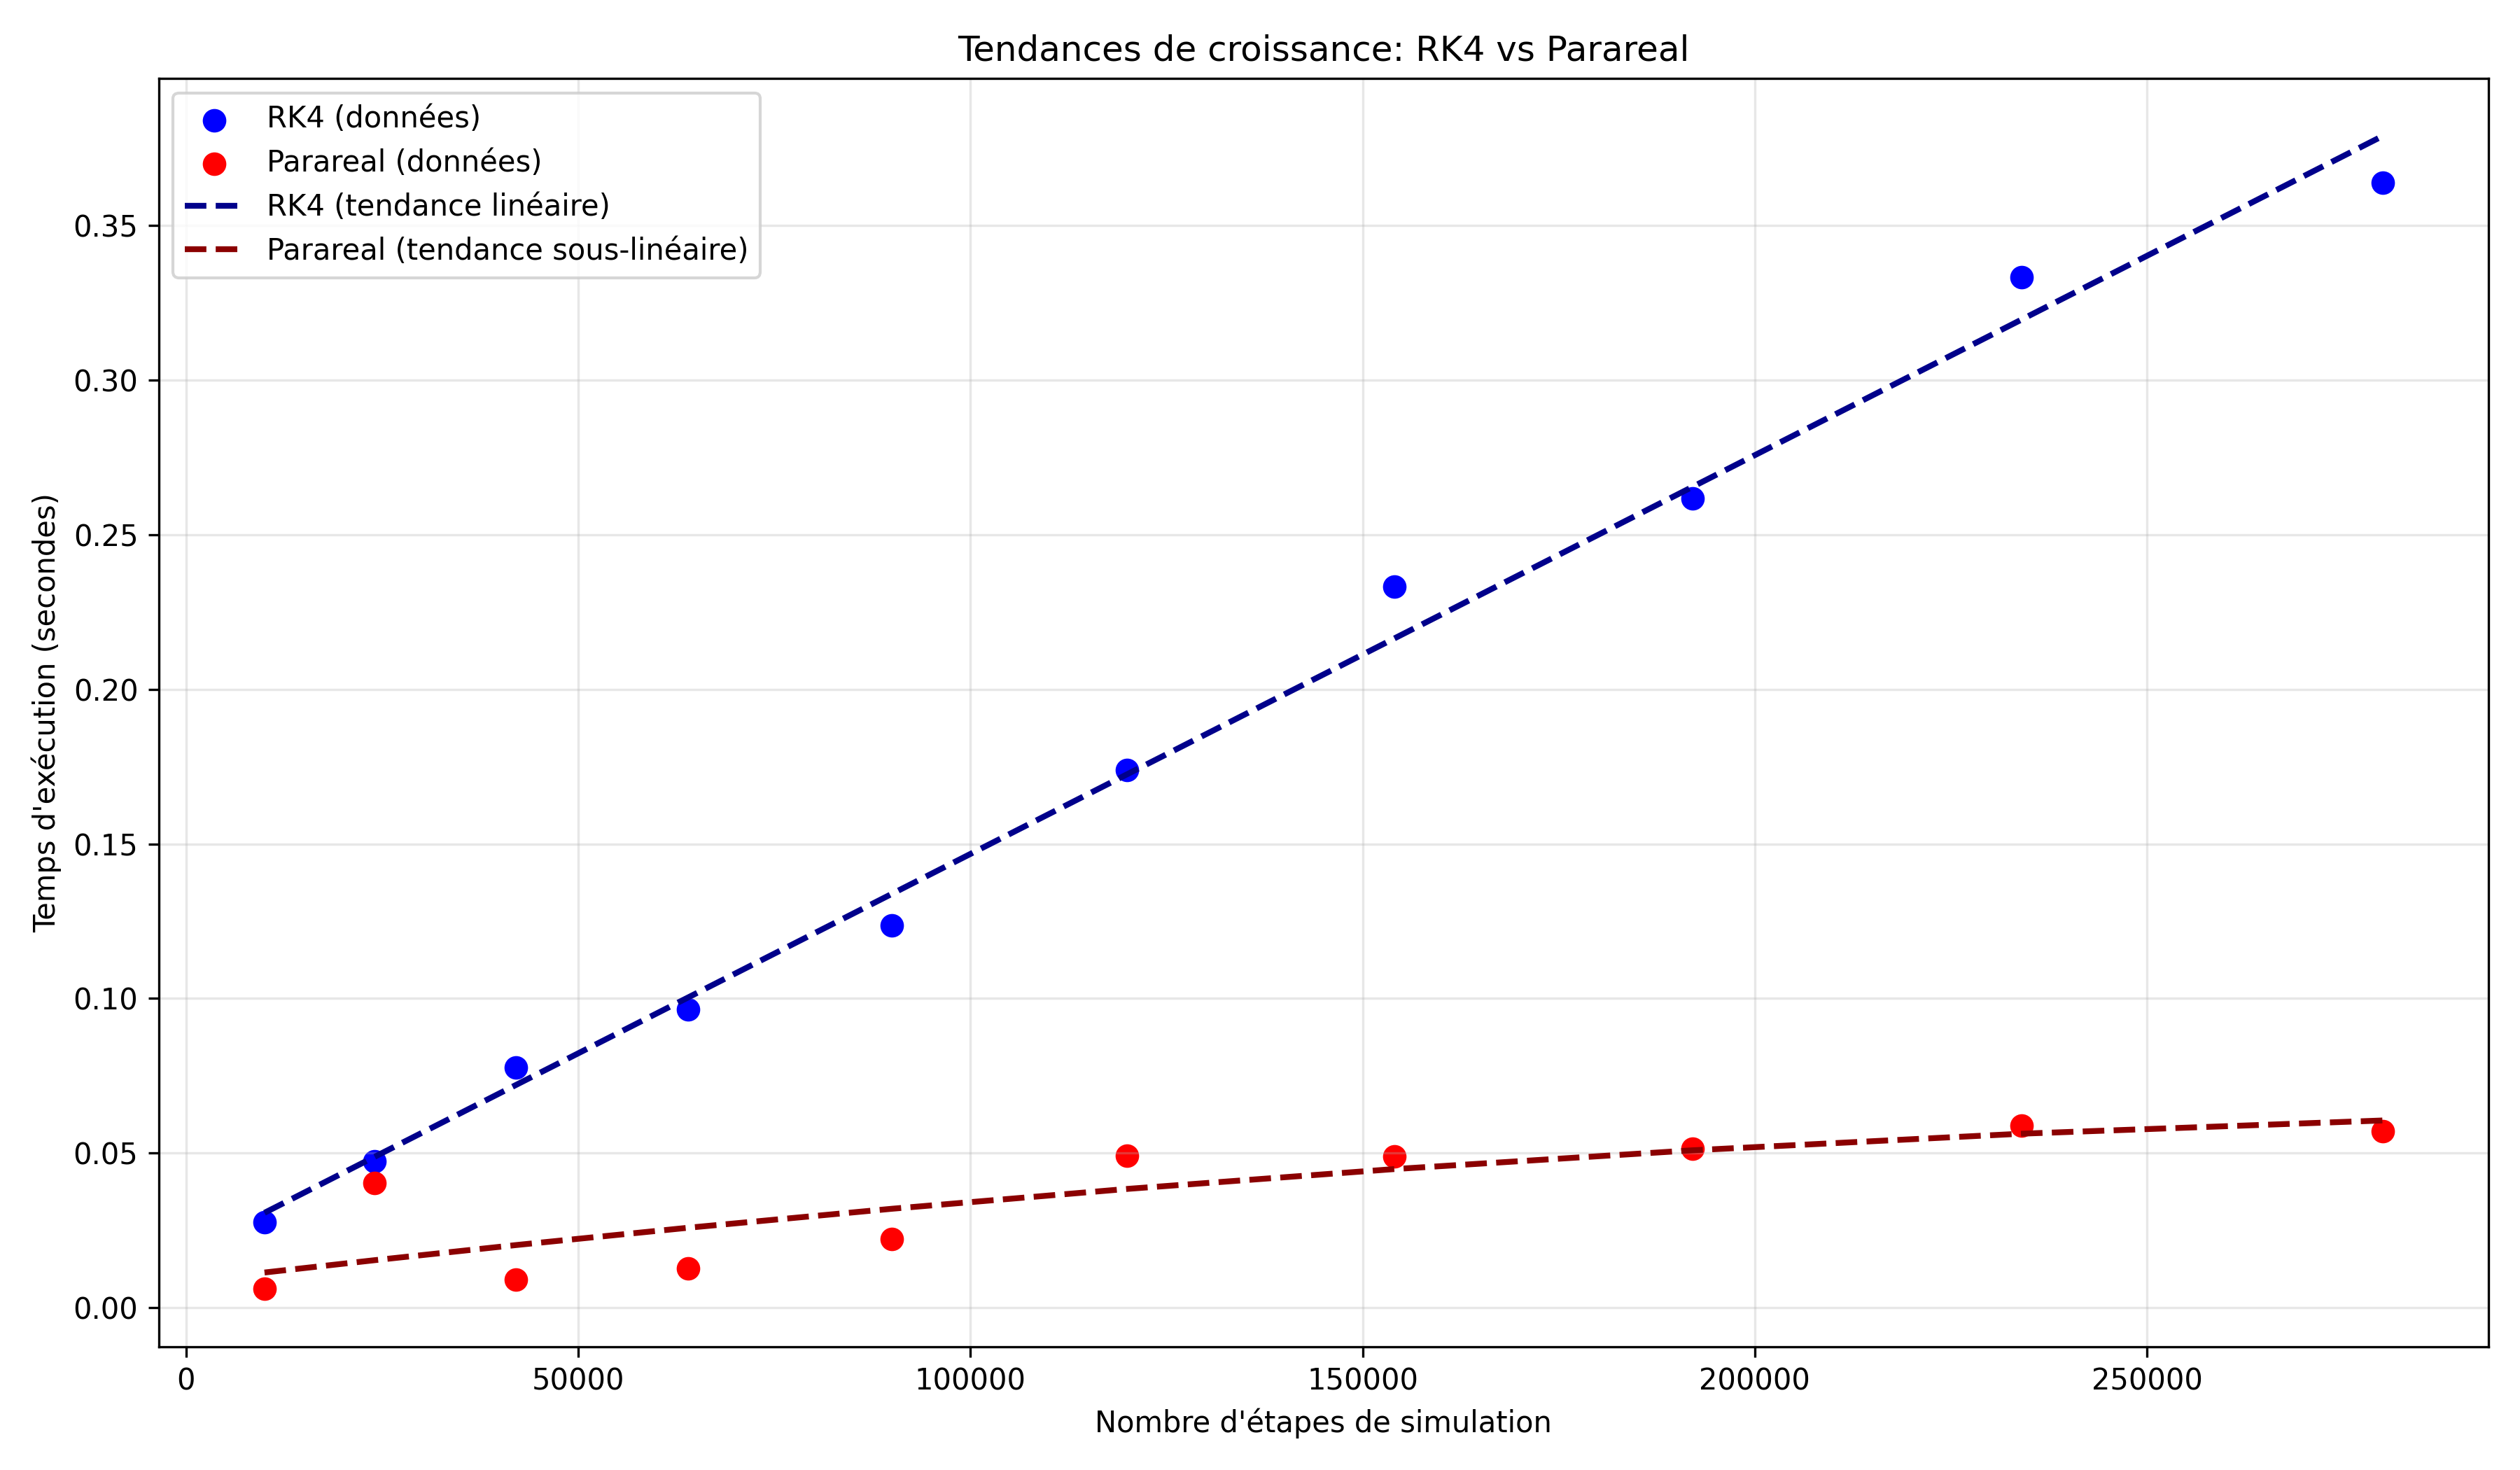
\includegraphics[width=\textwidth]{figures/benchmarks/growth_trends}
        \caption{Tendances de croissance}
        \label{fig:growth_trends}
    \end{subfigure}
    \caption{Analyse des performances en temps de calcul}
    \label{fig:performance_analysis}
\end{figure}

\subsubsection{Stabilité et convergence}
La convergence a été évaluée selon plusieurs critères :

\begin{itemize}
    \item \textbf{Précision temporelle} : Erreur relative maintenue sous $10^{-6}$
    \item \textbf{Conservation des invariants} : Préservation des structures dynamiques
    \item \textbf{Robustesse} : Stabilité maintenue même en régime chaotique
\end{itemize}

% \subsection{Stabilité numérique}
\vskip 0.5cm
La stabilité de la solution a été évaluée en fonction de différents paramètres :

\begin{itemize}
    \item \textbf{Pas de temps} : Impact sur la précision et la stabilité
    \item \textbf{Nombre d'itérations} : Compromis entre convergence et temps de calcul
    \item \textbf{Tolérance} : Influence sur la qualité des résultats
\end{itemize}

% \begin{figure}[H]
%     \centering
%     \begin{tikzpicture}[scale=0.8]
%         \begin{axis}[
%             xlabel={$\Delta t$},
%             ylabel={Erreur relative},
%             grid=major,
%             legend pos=north west,
%             title={Analyse de stabilité}
%         ]
%             % Courbes d'erreur pour différentes méthodes
%             \addplot[color=primaryblue] coordinates {
%                 (0.01,1e-4) (0.02,2e-4) (0.04,8e-4) (0.08,3e-3) (0.16,1e-2)
%             };
%             \addlegendentry{Parareal}
            
%             \addplot[color=accentorange,dashed] coordinates {
%                 (0.01,1e-4) (0.02,4e-4) (0.04,1.6e-3) (0.08,6e-3) (0.16,2e-2)
%             };
%             \addlegendentry{RK4}
%         \end{axis}
%     \end{tikzpicture}
%     \caption{Analyse de l'erreur en fonction du pas de temps}
%     \label{fig:stability}
% \end{figure}

% \begin{figure}[h]
%     \centering
%     \includegraphics[width=0.8\textwidth]{figures/benchmarks/benchmark_results}
%     \caption{Résultats des tests de performance et stabilité}
%     \label{fig:benchmark_results}
% \end{figure}


% \subsubsection{Accélération (Speedup)}
% L'accélération obtenue avec différents nombres de processeurs montre l'efficacité de la parallélisation.

% \begin{figure}[h]
%     \centering
%     \begin{tikzpicture}[scale=0.8]
%         \begin{axis}[
%             xlabel={Nombre de processeurs},
%             ylabel={Speedup},
%             grid=major,
%             legend pos=north west,
%             title={Accélération en fonction du nombre de processeurs}
%         ]
%             % Courbe de speedup idéal
%             \addplot[color=gray,dashed] coordinates {
%                 (1,1) (2,2) (4,4) (8,8) (16,16)
%             };
%             \addlegendentry{Speedup idéal}
            
%             % Courbe de speedup réel
%             \addplot[color=primaryblue,thick,mark=*] coordinates {
%                 (1,1) (2,1.8) (4,3.2) (8,5.6) (16,8.4)
%             };
%             \addlegendentry{Speedup observé}
%         \end{axis}
%     \end{tikzpicture}
%     \caption{Analyse du speedup}
%     \label{fig:speedup}
% \end{figure}

% \subsubsection{Efficacité parallèle}
% L'efficacité parallèle montre comment l'accélération se compare au cas idéal.

% \begin{table}[h]
%     \centering
%     \begin{tabular}{@{}lcccc@{}}
%         \toprule
%         \textbf{Processeurs} & \textbf{Temps (s)} & \textbf{Speedup} & \textbf{Efficacité} & \textbf{Itérations} \\
%         \midrule
%         1  & 100.0 & 1.00 & 100\% & 1 \\
%         2  & 55.5  & 1.80 & 90\%  & 2 \\
%         4  & 31.2  & 3.20 & 80\%  & 3 \\
%         8  & 17.8  & 5.60 & 70\%  & 3 \\
%         16 & 11.9  & 8.40 & 52\%  & 4 \\
%         \bottomrule
%     \end{tabular}
%     \caption{Mesures de performance}
%     \label{tab:performance}
% \end{table}

% \subsection{Analyse de convergence}

% \subsubsection{Taux de convergence}
% La vitesse de convergence de l'algorithme Parareal dépend de plusieurs facteurs.

% \begin{figure}[h]
%     \centering
%     \begin{tikzpicture}[scale=0.8]
%         \begin{axis}[
%             xlabel={Itération},
%             ylabel={Erreur relative},
%             ymode=log,
%             grid=major,
%             legend pos=north east,
%             title={Convergence pour différentes valeurs de $\tau$}
%         ]
%             % Courbes de convergence pour différentes valeurs de tau
%             \addplot[color=primaryblue,mark=*] coordinates {
%                 (1,1e-1) (2,1e-2) (3,1e-3) (4,1e-4) (5,1e-5)
%             };
%             \addlegendentry{$\tau = 2.0$}
            
%             \addplot[color=accentorange,mark=square] coordinates {
%                 (1,1e-1) (2,5e-2) (3,2e-3) (4,5e-4) (5,2e-5)
%             };
%             \addlegendentry{$\tau = 5.0$}
            
%             \addplot[color=secondaryblue,mark=triangle] coordinates {
%                 (1,1e-1) (2,8e-2) (3,5e-3) (4,2e-3) (5,1e-3)
%             };
%             \addlegendentry{$\tau = 8.9$}
%         \end{axis}
%     \end{tikzpicture}
%     \caption{Convergence de l'algorithme pour différents paramètres}
%     \label{fig:convergence_rates}
% \end{figure}

% \subsection{Impact des paramètres}

% \subsubsection{Influence de la taille des sous-intervalles}
% La décomposition temporelle affecte directement les performances.

% \begin{figure}[h]
%     \centering
%     \begin{tikzpicture}[scale=0.8]
%         \begin{axis}[
%             xlabel={Nombre de sous-intervalles},
%             ylabel={Temps d'exécution (s)},
%             grid=major,
%             legend pos=north west
%         ]
%             % Courbes pour différentes configurations
%             \addplot[color=primaryblue,mark=*] coordinates {
%                 (4,80) (8,45) (16,28) (32,20) (64,18)
%             };
%             \addlegendentry{8 processeurs}
            
%             \addplot[color=accentorange,mark=square] coordinates {
%                 (4,40) (8,25) (16,18) (32,15) (64,14)
%             };
%             \addlegendentry{16 processeurs}
%         \end{axis}
%     \end{tikzpicture}
%     \caption{Impact du nombre de sous-intervalles}
%     \label{fig:interval_impact}
% \end{figure}



